\section{Solar Calibrated Stellar Models}\label{sec:SCSM}
% In order to further validate the OPLIB high-temperature opacities we first visually
% compare a set of opacity vs. temperature curves from OPLIB at a constant $R$
% and \citet{Grevesse1998} composition (GS98) to the same curve from OPAL. A
% characteristic opacity vs temperature curve is shown in Figure
% \ref{fig:OpacCompare}, $\log _{10}(R) = -1.5$ is chosen as for much of the
% radius of a main sequence star $\log _{10}(R)$ is around that value. The
% largest variation in $\kappa_{R}$ from OPAL to OPLIB at $\log _{10}(R)=-1.5$ is
% on the order of a few percent. This is inline with expectations of OPLIB and OPAL
% being in relatively close agreement \citep{Colgan2016}.


In order to validate the OPLIB opacities, we generate a solar calibrated
stellar model (SCSM) using these new tables. We allow both the convective
mixing length parameter, $\alpha_{ML}$, and the initial Hydrogen mass fraction,
$X$, to vary simultaneously, minimizing the difference between resultant
models' final radius and luminosity to those of the sun.

Optimization of $\alpha_{ML}$ and $X$ is conducted using gradient descent. For
each optimization step three models are evolved: a reference model, a model
with a small perturbation to the hydrogen mass fraction but the same mixing
length as the reference model, and a model with a small perturbation to the
mixing length but the same hydrogen mass fraction as the reference.
Perturbations are sampled from a normal distribution (using
\texttt{numpy.random}). This distribution is sampled and that sample is then
added to the reference value for either $X$ or $\alpha_{ML}$. The luminosity
and radius of the three evolved models are compared to solar values and the
gradient of the resultant $L-L_{\odot}$, $R-R_{\odot}$ surface is followed down
to new estimates for the reference values of $X$ and $\alpha_{ML}$. This
process is is repeated until the difference between successive $X$ and
$\alpha_{ML}$ drops below one part in $10^{5}$.

\begin{figure}
	\centering
	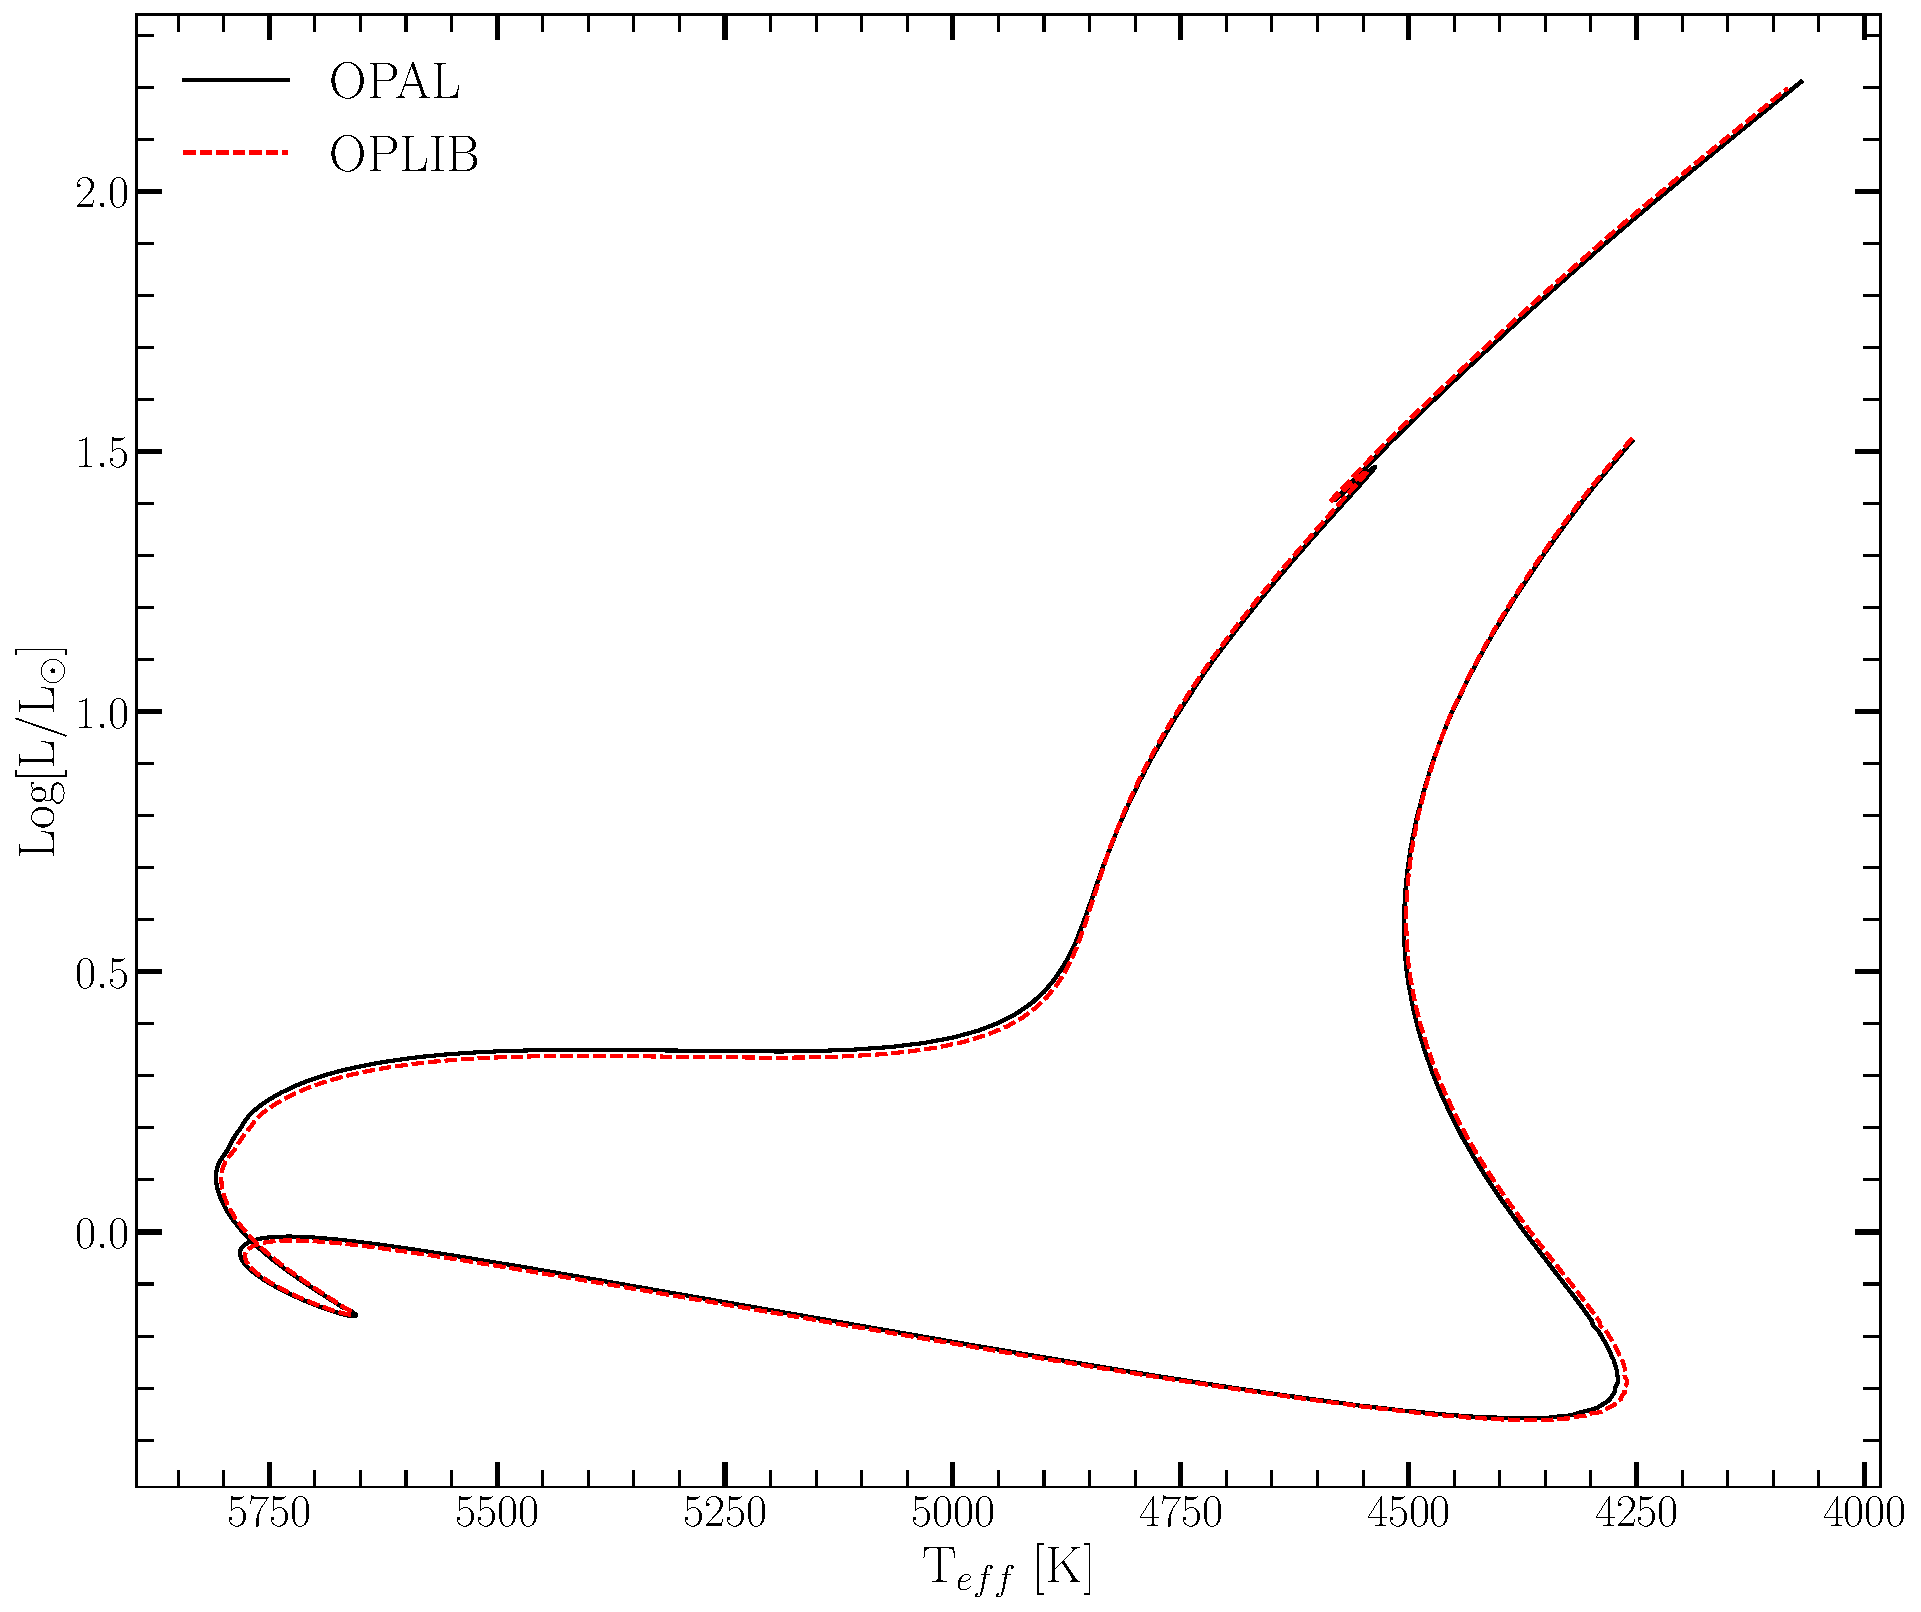
\includegraphics[width=0.45\textwidth]{src/figures/NotebookFigs/HRDiagramOPALvsOPLIB_SCCM.pdf}
	\caption{HR Diagram for the two SCSMs, OPAL and OPLIB. OPLIB is shown as a grey
	dashed line.}
	\label{fig:OPLIBOPALHR}
\end{figure}

Solar calibrated stellar models evolved using GS98 OPAL and OPLIB opacity
tables (Figure \ref{fig:OPLIBOPALHR}) differ $\sim 0.5\%$ in the SCSM hydrogen
mass fractions and $\sim 1.5\%$ in the SCSM convective mixing length parameters
(Table \ref{tab:SCSMResults}). While the two evolutionary tracks are very
similar, note that the OPLIB SCSM's luminosity is systematically lower at the
same age until the star leaves the main sequence, at which point it is
effectively the same as the OPAL SCSM. This luminosity difference between OPAL
and OPLIB based models is consistent with expectations given the shallow
radiative temperature gradient resulting from the lower OPLIB opacities

\begin{table}
	\centering
	\begin{tabular}{l c c}
		\hline
		Model & $X$ & $\alpha_{ML}$ \\
		\hline
		\hline
		OPAL & 0.7066 & 1.9333 \\
		OPLIB & 0.7107 & 1.9629
	\end{tabular}
	\caption{Optimized parameters for SCSMs evolved using OPAL and OPLIB high
	temperature opacity tables.}
	\label{tab:SCSMResults}
\end{table}
